\textbf{What is cryptocurrency?}

A cryptocurrency, crypto-currency, or crypto is a digital currency designed to work as a medium of exchange through a computer network that is not reliant on any central authority, such as a government or bank, to uphold or maintain it.

Individual coin ownership records are stored in a digital ledger, which is a computerized database using strong cryptography to secure transaction records, to control the creation of additional coins, and to verify the transfer of coin ownership. Despite their name, cryptocurrencies are not considered to be currencies in the traditional sense and while varying treatments have been applied to them, including classification as commodities, securities, as well as currencies, cryptocurrencies are generally viewed as a distinct asset class in practice.Some crypto schemes use validators to maintain the cryptocurrency. In a proof-of-stake model, owners put up their tokens as collateral. In return, they get authority over the token in proportion to the amount they stake. Generally, these token stakers get additional ownership in the token over time via network fees, newly minted tokens or other such reward mechanisms.
Cryptocurrency does not exist in physical form like paper money and is typically not issued by a central authority. Cryptocurrencies typically use decentralized control as opposed to a central bank digital currency (CBDC).When a cryptocurrency is minted or created prior to issuance or issued by a single issuer, it is generally considered centralized. When implemented with decentralized control, each cryptocurrency works through distributed ledger technology, typically a blockchain, that serves as a public financial transaction database.Traditional asset classes like currencies, commodities, and stocks, as well as macroeconomic factors, have modest exposures to cryptocurrency returns.
The first decentralized cryptocurrency was Bitcoin, which first released as open-source software in 2009. As of March 2022 there were more than 9,000 other cryptocurrencies in the marketplace, of which more than 70 had a market capitalization exceeding 1 billion.

\begin{figure}[H]
\centering

\includegraphics[width=0.2\textwidth]{images/btclogo.png}
\caption{A logo for Bitcoin, the first decentralized cryptocurrency}
\label{fig:bitcoin}
\end{figure}

\begin{figure}[H]
\centering
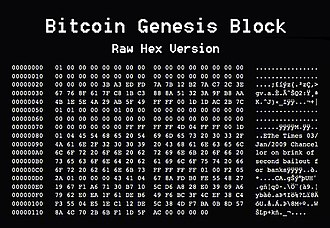
\includegraphics[width=0.5\textwidth]{images/Bitcoin-Genesis-block.jpg}
\caption{The genesis block of Bitcoin's blockchain, with a note containing The Times newspaper headline. This note has been interpreted as a comment on the instability caused by fractional-reserve banking.}
\label{fig:bitcoin-genesis-block}
\end{figure}

\textbf{Purposes of this paper}

Cryptocurrencies are a new asset class that is not yet widely used in the market. The purpose of
this paper is to explore the potential uses of cryptocurrencies in the markets. How we can generate
crypto assets and potentially use this currency in the market and in our life?
Note this paper is written in a South African context, some of the ideas mentioned in the paper
are not applicable to the rest of the world. Different countries have different laws and regulations on
the use of cryptocurrencies.
I have tested all methodologies in this paper and implemented code to automate my stock market
investments. Source Code will not be provided for auto trading bots but resources and manuals will
be provided for you to use them, To implement automation of trading. \\

\textbf{Paper Objectives}

\begin{enumerate}
\item Introduce the concept of a crypto wallet.
\item Introduce the concept of generating crypto assets by mining (Passive Income).
\item Convert your crypto assets to fiat currency.
\item Taxation laws for cryptocurrency in South Africa.
\item Using cryptocurrency in selected stores without fiat currency.
\item Converting crypto to fiat then using a debit order for stock market investments.
\end{enumerate}


 